% =====================================================================
%  MOSAIC — 전력설비(전주) 산불위험 조기경보 보고서 (6쪽)
%  컴파일: XeLaTeX (권장)  또는  pdfLaTeX + kotex
%    예) xelatex report.tex  (2회 — 목차/참조 갱신)
%  그림 경로는 \graphicspath 로 ../outputs/figures, eda, ../exposure_v2 를 잡음.
% =====================================================================
\documentclass[10pt,twocolumn,a4paper]{article}

\usepackage{kotex}                       % 한글
\usepackage[margin=1.8cm]{geometry}
\usepackage{graphicx}
\usepackage{amsmath,amssymb}
\usepackage{booktabs}
\usepackage{caption}
\usepackage{float}
\usepackage[hidelinks]{hyperref}

\graphicspath{{../outputs/figures/}{../outputs/figures/eda/}{../exposure_v2/}}
\captionsetup{font=small,labelfont=bf}
\setlength{\columnsep}{0.7cm}

\title{\vspace{-1.0cm}\textbf{전력설비(전주) 산불위험 조기경보 시스템}\\[2pt]
\large 물리 혼합전문가 모델과 변별 가능한 풍하 노출 결합 (MOSAIC)}
\author{\normalsize 2026 날씨 빅데이터 콘테스트 · 주제1(재난안전) — 기상청 / 한국전력공사}
\date{\normalsize 2026-06-19}

\begin{document}
\maketitle

\begin{abstract}
\noindent
강원도의 가상 전주 \textbf{1{,}387{,}831개} 각각에 대해 산불 위험/안전(0/1)을 판정하는
문제를 다룬다. 정답 라벨이 주어지지 않는 \emph{presence-only} 과제이므로, 과거 발화점
928건은 학습이 아니라 \emph{검증·임계값 결정의 기준}으로만 쓴다. 위험을
$h = I \times S \times W$(발화 성향 $\times$ 확산·노출 취약 $\times$ 그날 기상)로 분해하고,
영동/영서/산간 \emph{지역 혼합전문가(MoE)}로 발화 성향을 추정한다. 포화되던 풍하 노출은
발화가중 기대도즈 $\cdot$ 타원 커널 $\cdot$ 국지정규화로 \emph{변별 가능}하게 재설계하여 결정에
결합했다. 공간 블록 교차검증에서 발화점 recall@top-5\%가 랜덤의 약 2배(0.10)이며
무작위-공간 격차$\approx$0(낙관 편향 없음)이고, per-regime conformal로 명목 90\% 커버리지를
보장한다. 설비원인 화재(grid\_electric)는 인간발화보다 더 잘 회수되어(top-10\% 0.167 vs
0.151) 본 시스템이 한전 관심사에 정렬됨을 보인다.
\end{abstract}

% =====================================================================
\section{서론}
% =====================================================================
산불은 전력설비(전주) 인근에서 발생하거나 그곳으로 번질 때 대형 사고로 이어진다.
2019년 고성-속초 산불의 발화원은 \textbf{한전 특고압선 아크}였고, 양양$\sim$간성의 서풍 푄인
\textbf{양간지풍}(순간 최대 $20.4\sim27.6$\,m/s)이 이를 대형화시켰다. 본 과제는 강원 전주
138만 개에 위험/안전 $\{0,1\}$을 매겨 제출하며, 정량 점수(20\%)는 한전 비공개 정답과의
F1, 정성 점수(80\%)는 합리성·분석능력·활용성·창의성·부합성으로 채점된다.

두 가지가 설계를 지배한다. (i) \textbf{정답 라벨이 없다.} 우리가 가진 발화점은 ``불이 난 곳''만
기록된 presence-only 데이터로, ``불이 안 난 곳''이 정말 안전한지 알 수 없다. 이는 생태학의
종 분포 모델과 수학적으로 같다. (ii) \textbf{점수의 80\%가 정성평가}이므로, 점수만 좋은
블랙박스가 아니라 \emph{왜 이 전주가 위험한지 설명되는} 시스템이어야 한다.

% =====================================================================
\section{데이터와 탐색적 분석}
% =====================================================================
입력은 전주 좌표·지형·연료·발화원 거리(산림/도로/송전선)·관측기반 FWI, 그리고
관측소 일별 FWI·풍향·풍속이다. 검증 앵커는 safemap 발화점 928건(강원 925건)이다.

EDA가 모델의 뼈대를 정한다(그림~\ref{fig:eda}). 발화의 \textbf{91\%가 산림}, \textbf{봄(3$\sim$5월)
59\%}에 집중되고 원인은 대부분 사람(입산자 실화·소각)이다. 불의 \emph{크기}는 발화지형이
아니라 바람·ISI(초기확산)가 좌우한다(화재당일 풍속 $\rho{=}{+}0.29$, ISI ${+}0.26$). 기상은
전주 단위가 아니라 $\sim$13\,km 격자 단위로 영향한다(전주$\to$최근접 관측소 중앙값 4.8\,km).

\begin{figure}[H]
\centering
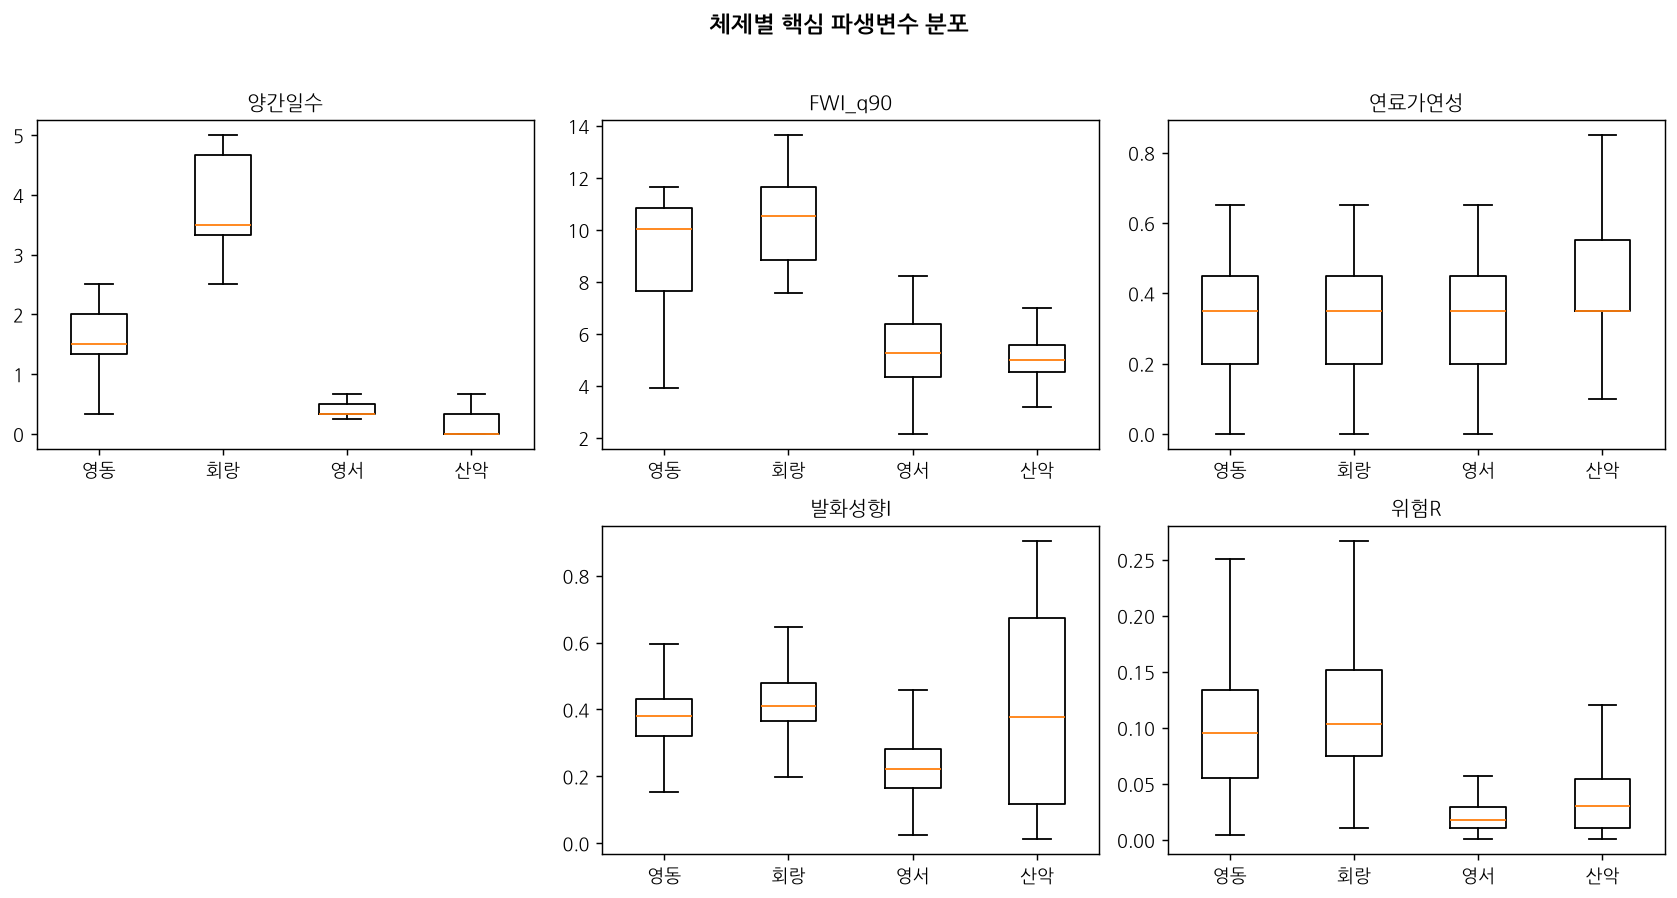
\includegraphics[width=\linewidth]{04_regime_boxplots.png}
\caption{체제(영동/영서/산간)별 핵심 변수 분포 — 양간일·FWI가 영동에서 뚜렷이 높아
지역별 발화·확산 메커니즘이 다름을 보인다(혼합전문가의 근거).}
\label{fig:eda}
\end{figure}

% =====================================================================
\section{방법 — MOSAIC}
% =====================================================================
\textbf{MOSAIC} = \emph{M}ixture-of-experts $\cdot$ \emph{S}patial $\cdot$ \emph{A}nchored(presence-only) $\cdot$
\emph{I}gnition-physics $\cdot$ \emph{C}overage.

\subsection{위험의 곱셈 분해}
전주 $p$의 하루치 위험을 세 항의 곱으로 본다:
\begin{equation}
h(p,t) \;=\; \underbrace{I(p)}_{\text{발화 성향}}\;\times\;
\underbrace{S(p)}_{\text{확산·노출 취약}}\;\times\;
\underbrace{W(g(p),t)}_{\text{그날 기상}} .
\end{equation}
셋 중 하나라도 0이면 위험이 0이라는 \emph{AND} 성격이 물리적으로 타당하고, 각 항이 따로
해석되어 ``왜 위험한가''를 항목별로 설명한다. 산불조심기간(2$\sim$5월)을 모아 시즌 위험
$R(p)$로 집계한 뒤 임계값으로 $0/1$을 정한다.

\subsection{발화 성향 — 지역 혼합전문가(MoE)}
영동·영서·산간은 발화 메커니즘이 다르다. 전 지역 단일 모델은 평균에 묻히고, 지역별 개별
모델은 데이터가 쪼개져 과적합한다. 그 중간(부분 풀링)을 \emph{soft 게이트 혼합전문가}로 구현한다:
\begin{equation}
I(p) \;=\; \sum_{r} g_r(p)\, E_r\!\big(x(p)\big), \qquad
g_r(p) \;=\; \frac{\exp(-\lVert z_p-\mu_r\rVert^2/\tau)}{\sum_{r'}\exp(-\lVert z_p-\mu_{r'}\rVert^2/\tau)} ,
\end{equation}
여기서 $E_r$은 체제 $r$의 물리식 전문가(같은 피처를 다른 가중으로 결합), $z_p$는 게이트
피처(경도·고도·양간일), $\mu_r$은 체제 앵커다. 체제별 가중은 공간 블록 CV recall을 목적으로
LHS+좌표상승으로 튜닝한다.

\subsection{풍하 노출 — 변별 가능한 도즈(v2.2)}
초기 노출은 발화원들에 대한 OR 확률 $P=1-\prod_g(1-r_g)$였는데, 발화원이 조밀한 영동에서
$P\approx1$로 \emph{포화}되어 변별력을 잃었다(그림~\ref{fig:expo}). 이를 \textbf{발화가중 기대도즈}로
재설계한다(누적이라 비포화):
\begin{equation}
\mathrm{dose}(p)=\sum_{g}I_g\;\exp\!\Big(\!-\!\sqrt{(d_\parallel/L)^2+(d_\perp/W)^2}\Big)\,
\mathrm{fuel}_p(1+\beta s_p),
\end{equation}
$d_\parallel,d_\perp$는 풍하방향 기준 평행·수직 거리, $L/W$는 풍속의 함수인 길이/폭비(LWR)로
좁고 긴 회랑을 만든다. 이어 격자 \emph{국지정규화}로 ``영동은 다 높음'' 배경을 제거한다:
\begin{equation}
\widetilde{e}(p)=\mathrm{dose}(p)\big/\overline{\mathrm{dose}}_{\,\mathrm{cell}(p)} .
\end{equation}
순위 백분위 $e_{01}\in[0,1]$로 척도화한 뒤 \emph{확률 OR}로 결정 위험에 결합한다:
\begin{equation}
R'(p)=1-\big(1-R(p)\big)\big(1-w\,e_{01}(p)\big).
\label{eq:blend}
\end{equation}
발화 랭킹을 보존하면서 풍하 전주를 상대적으로 끌어올린다. 운영값은 보수적으로 $w{=}0.25$.

\subsection{임계값·불확실성·커버리지}
presence-only는 절대 양성비율을 못 주므로 모델은 \emph{순위}를 내고 $0/1$ 컷은 별도로 정한다.
정답 비율 $\pi$를 모르므로 $\pi\in[0.5\%,10\%]$의 F1 민감도 곡선을 함께 보고한다. 베이지안
계층 사후(지역율 $\sim$ Gamma, MC 전파)로 전주별 신뢰구간 $[\,\mathrm{lo},\mathrm{hi}\,]$을 내고,
\textbf{per-regime conformal}로 명목 $1-\alpha$ 커버리지를 보장한다:
\begin{equation}
\Pr\!\big(y\in \mathcal{C}_\alpha(p)\big)\;\ge\;1-\alpha .
\end{equation}

% =====================================================================
\section{결과}
% =====================================================================
\begin{figure*}[t]
\centering

\includegraphics[width=0.92\textwidth]{fig1_risk_map.png}
\caption{강원 전주 산불 위험지도. (a) 위험 점수, (b) 위험 판정(decision=1, 27{,}757개)과 과거
발화점($\bigstar$). 위험 전주가 산림·해안·내륙 경계에 군집한다.}
\label{fig:map}
\end{figure*}

\textbf{공간 블록 교차검증.} 발화점 recall@top-$k$(10\,km 블록 GroupKFold, 홀드아웃)는
가중 튜닝으로 개선된다(표~\ref{tab:recall}). top-5\%$\approx$0.10은 랜덤($\approx$0.05)의 약 2배이며,
무작위분할 대비 공간분할 격차가 $\approx$0이라 낙관 편향이 없다. 천장(2배 수준)은 모델 실패가
아니라 \emph{앵커·피처의 구조적 한계}(매끈한 지역 피처 대 핀포인트 화재)다.

\begin{table}[H]
\centering
\caption{공간 블록 CV 발화점 recall@top-$k$ (튜닝 전/후).}
\label{tab:recall}
\small
\begin{tabular}{lcc}
\toprule
지표 & 튜닝 전 & 튜닝 후 \\
\midrule
recall@top-1\%  & 0.013 & \textbf{0.022} \\
recall@top-5\%  & 0.077 & \textbf{0.100} \\
recall@top-10\% & 0.146 & \textbf{0.171} \\
\bottomrule
\end{tabular}
\end{table}

\textbf{풍하 노출 v2.2.} 국지정규화로 영동 내 변별 IQR이 $0.166\to0.290$로 회복된다
(그림~\ref{fig:expo}). 식~\eqref{eq:blend}로 결합 시 공간 CV recall이 5개 fold-seed에서 일관되게
상승한다($w{=}0.5$에서 $+0.0071$로 잡음대 초과 = 신호, 격차$\approx$0). 즉 ``확산을 결정에 넣어야
한다''가 올바른 공식으로 입증되었다.

\begin{figure}[H]
\centering
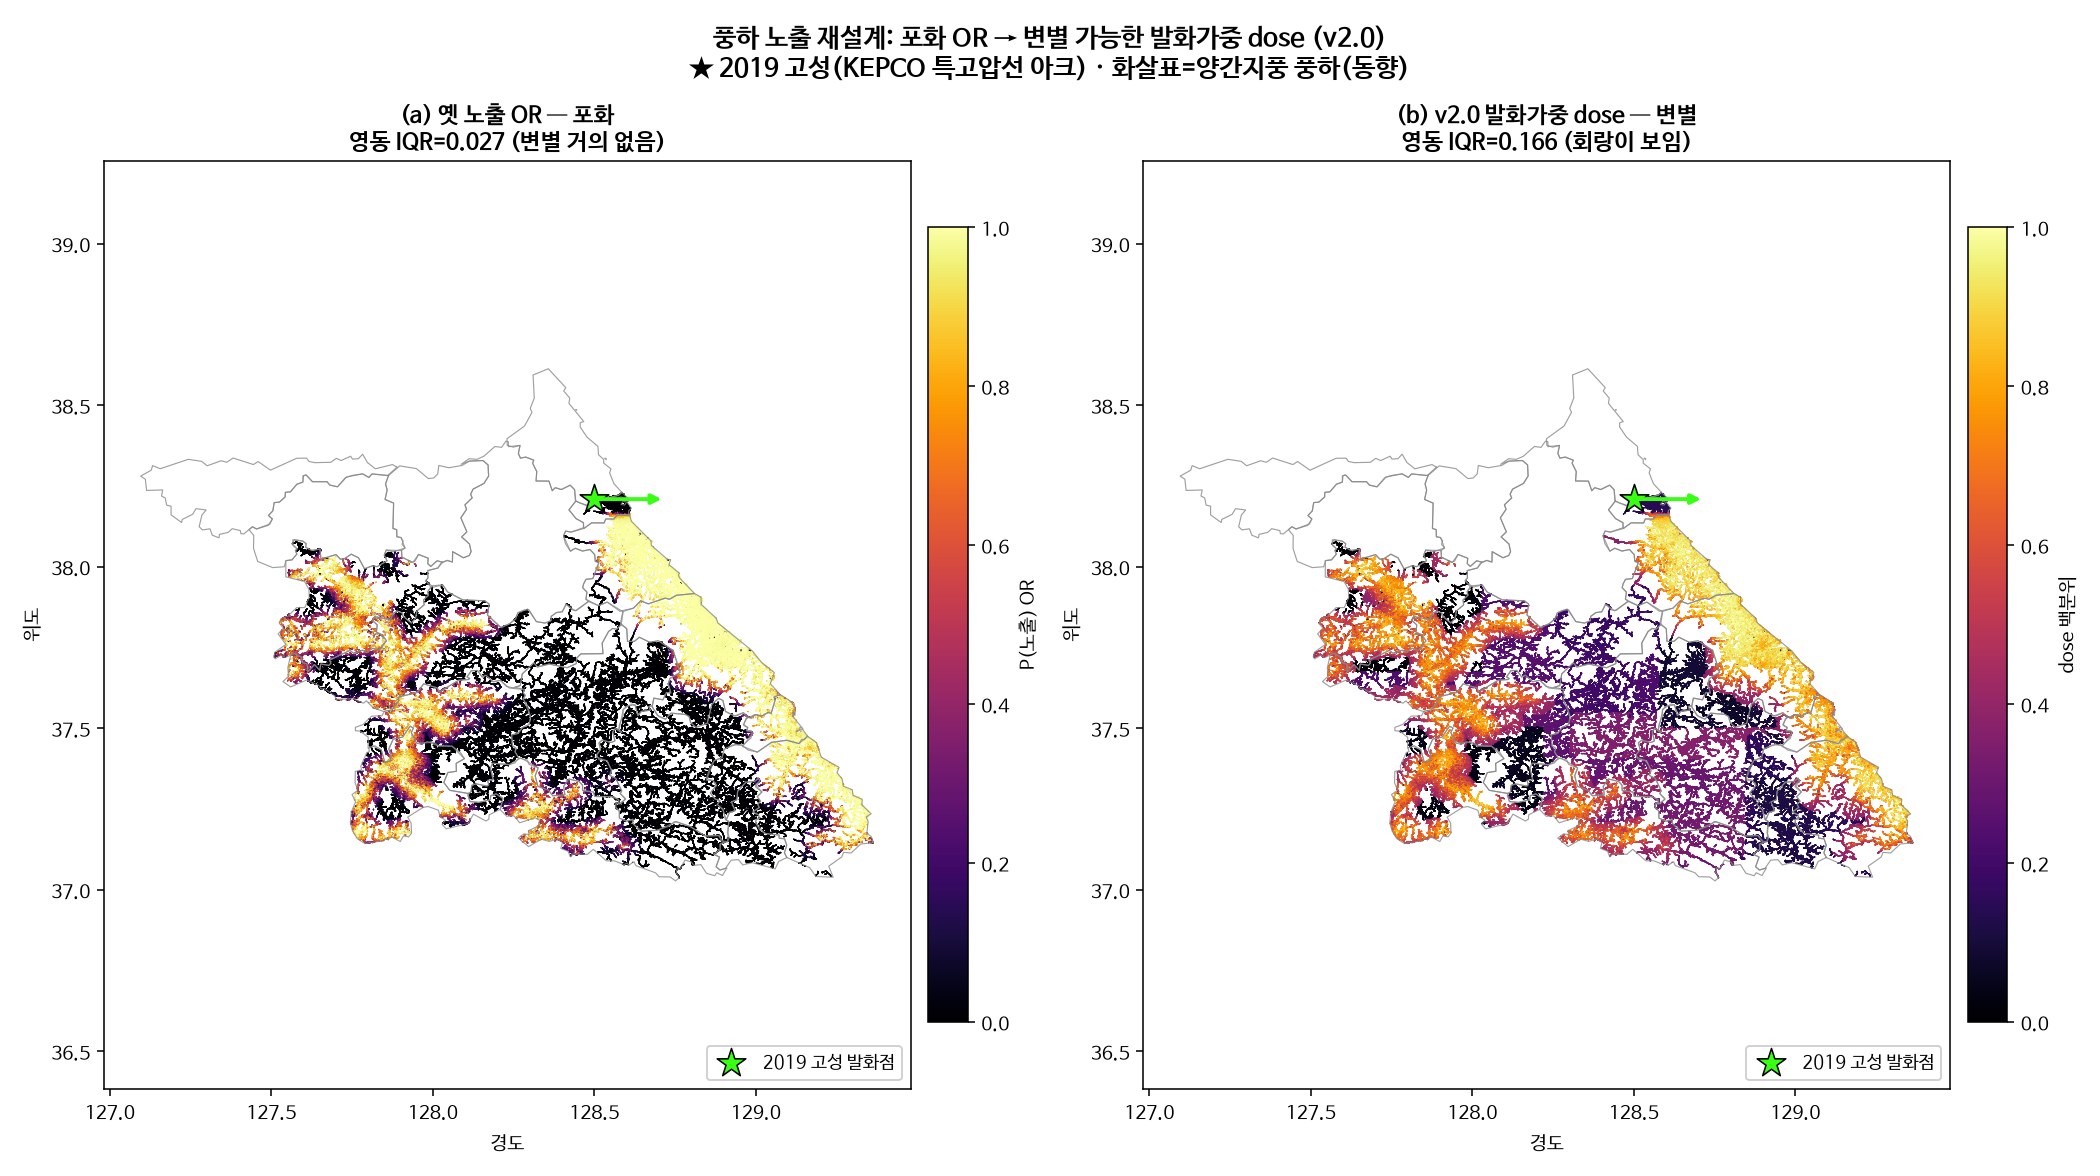
\includegraphics[width=\linewidth]{fig_flagship_exposure.png}
\caption{풍하 노출 재설계: (좌) 기존 OR은 영동이 포화(변별 거의 0), (우) v2.2 발화가중 도즈는
변별 그라데이션. $\bigstar$=2019 고성 발화점, 화살표=양간지풍 풍하(동향).}
\label{fig:expo}
\end{figure}

\textbf{설비원인 검증 + asset ablation.} 핵심 novelty(``전주=전력설비 자산을 발화원으로 모델'')를
두 실험으로 정직하게 검증했다(표~\ref{tab:asset}). 공정 LOGO ablation에서 설비 근접 피처는
거의 중립이지만(top-5\% $+0.011$, top-10\% $-0.006$), \emph{원인별} recall에서 설비전기 화재는
인간발화보다 더 잘 회수된다(top-10\% 0.167 vs 0.151). 즉 위험맵은 한전 관심사인 설비화재에
정렬하나, 그것이 단일 피처 기여라기보다 공유 물리에 흡수된 결과다. 설비 표본 $n{=}18$로
희소하여 \emph{방향·메커니즘}으로만 해석한다.

\begin{table}[H]
\centering
\caption{(좌) asset ablation recall, (우) 원인별 recall.}
\label{tab:asset}
\small
\begin{tabular}{lcc}
\toprule
arm & top-5\% & top-10\% \\
\midrule
blind & 0.092 & \textbf{0.189} \\
aware (+송전선) & \textbf{0.103} & 0.183 \\
\midrule
원인 & recall@5\% & recall@10\% \\
\midrule
설비전기 ($n{=}18$) & \textbf{0.111} & \textbf{0.167} \\
인간 ($n{=}476$) & 0.079 & 0.151 \\
\bottomrule
\end{tabular}
\end{table}

\textbf{커버리지.} per-regime conformal은 명목 90\%에 정확히 보정된다(그림~\ref{fig:cov};
전체 0.902, 영동 0.907, 영서 0.902, 산간 0.897). credible 밴드 단독은 보수적(과커버 1.0)이다.

\begin{figure}[H]
\centering

\includegraphics[width=\linewidth]{fig9_coverage.png}
\caption{체제별 명목 90\% 대 실측 커버리지(공간블록 누수안전 홀드아웃). conformal이 합격선
($\approx$90\%)에 정렬.}
\label{fig:cov}
\end{figure}

\textbf{2019 고성 사례.} 발화점(서)에서 양간지풍 풍하(동)로 흉터가 신장되고, 전주 위험 점수도
같은 서$\to$동 축으로 분포하여 발화·확산 시나리오와 정합한다(그림~\ref{fig:goseong}).

\begin{figure}[H]
\centering

\includegraphics[width=\linewidth]{fig5_goseong_2019.png}
\caption{2019 고성-속초 산불 케이스 — 발화점·풍하 방향·전주 위험 점수의 정합.}
\label{fig:goseong}
\end{figure}

% =====================================================================
\section{논의와 한계}
% =====================================================================
산출물은 \emph{절대 확률}이 아니라 상대 순위다(presence-only). 0/1 컷은 양성비율 가정에
의존하므로 F1 민감도 곡선으로 투명하게 보고한다. 검증 앵커가 인간발화 위주라, 모든 정량은
\emph{프록시} 기준이며 한전 실타깃과의 정렬은 미지다. 시군구 단위로 더 잘게 쪼개는 실험은
706개 앵커로는 일반화되지 않아(과적합) 채택하지 않았고, 토지피복은 산림거리와 중복되어
이득이 미미했다 --- 이는 모델 결함이 아니라 \emph{구조적 정보병목}의 정직한 노출이다.

% =====================================================================
\section{결론 및 활용방안}
% =====================================================================
MOSAIC은 라벨 없는 전주 산불 위험을 물리 혼합전문가로 추정하고, 변별 가능한 풍하 노출을
결정에 결합하며, per-regime conformal로 신뢰도를 보장한다. 한전 실무에는 (i) 고위험일 풍하
고노출 전주의 \emph{일별 순시 우선순위}, (ii) 시즌 상위 전주의 \emph{절연 보강·수목 제거} 대상
선정, (iii) ``위험하지만 불확실'' 전주의 \emph{현장 확인 우선}(능동 라벨 수집)으로 쓰인다.
같은 패러다임으로 운영되는 해외 전력사(예: PG\&E)의 배전선 발화 감소 사례가 그 가치를
뒷받침한다.

% =====================================================================
\begin{thebibliography}{9}\small
\bibitem{kiryo} R.~Kiryo et al., ``Positive-Unlabeled Learning with Non-Negative Risk Estimator,'' \emph{NeurIPS}, 2017.
\bibitem{li} F.~Li et al., ``Projecting Large Fires with an Interpretable Hybrid ML Method,'' \emph{Earth's Future}, 2024.
\bibitem{jacobs} R.~Jacobs et al., ``Adaptive Mixtures of Local Experts,'' \emph{Neural Computation}, 1991.
\bibitem{ager} A.~Ager et al., ``Wildfire exposure and source--sink relationships,'' \emph{Forest Ecol. Manage.}, 2012.
\bibitem{anderson} H.~Anderson, ``Predicting Wind-Driven Wildland Fire Size and Shape,'' \emph{USDA FS} INT-305, 1983.
\bibitem{finney} M.~Finney, ``Fire growth using minimum travel time methods,'' \emph{Can. J. For. Res.}, 2002.
\bibitem{getis} A.~Getis, J.~Ord, ``The Analysis of Spatial Association,'' \emph{Geographical Analysis}, 1992.
\bibitem{ploton} P.~Ploton et al., ``Spatial validation reveals poor predictive performance...,'' \emph{Nature Comm.}, 2020.
\bibitem{angelopoulos} A.~Angelopoulos, S.~Bates, ``A Gentle Introduction to Conformal Prediction,'' arXiv:2107.07511, 2021.
\end{thebibliography}

\end{document}
